%\vspace*{\subsecspace}
\section{GPU Scheduling Design}
\vspace*{\subsecspace}
\label{sec:design}

% When choosing what to run next on a GPU, we have many factors to consider: fairness, expected load, memory requirements, and if our choice will be a warm start.
A GPU scheduler has different considerations in mind than traditional CPU serverless scheduling.
We must allow for concurrent dispatches to an individual GPU, but ensure they do not compete for compute resources while running.
If there is insufficient memory, do we need to move memory off the device to relieve pressure, or do we need to remove a container?
Locality is still important, as a function will have better performance if a container for it already exists, but if the memory is off-device, the benefit is less.  
On systems with multiple GPUs, we must be aware that an existing container we have may not match the GPU that's available to run, and we cannot alter this attachment.
Finally, it must provide fair access to GPU time and prevent starvation amongst all functions.

\subsection{Multi-Queue Fair Queuing}
\label{sec:queuing}

We take inspiration from MQFQ to ensure fairness between functions, but our design and implementation differ significantly to fit the new paradigm we are applying it to.
Our worker maintains a single queue structure from which it accomplishes these goals by tracking GPU utilization, function's usage of GPUs, and naturally, queuing and dispatching invocations.
Dispatches to GPUs are not as frequent as disk I/O, so its highly distributed structure isn't needed for throughput, and the contention over split resources would become excessive.
With this, each flow no longer dispatches independently of each other, so we must encourage locality by repeatedly dispatching from the same flow.
This case simply imitates a FCFS policy and serializes the flows into several queues.


% A new invocation is inserted into it's function's unique \emph{flow} on the worker, as shown in \circled{1} of Figure~\ref{fig:sys-diag}.
Each function is given a unique \emph{flow} on the worker, as shown in \circled{1} of Figure~\ref{fig:sys-diag}.
An invocation is inserted into its respective flow, and while non-empty, a flow is considered \emph{active}.
When the number of outstanding invocations is less than maximum \D for a GPU, we choose a flow and send its first item to execute.
This \D does not have to be fixed, and can vary with function usage of devices resources, and is described in detail below.
% A flow can be dispatched from successively up to \T times, at which point it is \emph{throttled} for fairness' sake.
On each dispatch, the flow's virtual time (VT) is incremented to denote time spent on device. 
Once a flow is \T dispatches ahead of the minimum VT of all flows, it is \emph{throttled} for fairness' sake.

% Each flow with invocations in it is considered \emph{active}, and is tracked with a virtual time equal to the minimum VT of all its enqueued invocations.
When inserted, they are assigned a virtual time (VT): the first entry uses the global VT, and future additions are assigned the max VT of all entries in the flow plus the average execution time of its representative function.
Functions are thus in ascending order of their VTs within the flow, and dispatched in FCFS order.
% Each unique function is mapped to a \emph{flow} in the system, which each have their own virtual time.
We prefer the function's execution time over a fixed increment because functions spend different amounts of wall time on the GPU, a fixed time would benefit longer functions to the detriment of short.
A flow's VT is given by the minimum VT of all its entries, and the global VT is the minimum of across all flows that are non-empty.
% Each flow's VT is the minimum VT of all the invocations waiting in it, and when emptied (made \emph{inactive}), it keeps the VT of the last entry.

To dispatch invocations, our GPU queue first checks if a GPU is available to run something step \circled{2} in Figure~\ref{fig:sys-diag}, and if so we acquire a token from the GPU manager (section~\ref{sec:gpu-man}) allowing access to a specific device.
Querying the GPU manager is required because functions may use only a portion of GPU resources, so we vary the number of tokens with pressure to enable higher concurrency.
% Once we have a token, we look at each flow whose $VT_{flow} < VT_{global} + VT_{thresh}$, i.e. flows that aren't throttled, and choose the flow with the lowest VT that also has a container on the GPU we are running our item on.
% If none match this condition, the lowest VT flow is chosen, and we accept that we must cold start a container.
To choose a flow, we pick the one with the minimum VT, but will override this with a preference to an active flow which has a container already warmed.
\todo{Change based on best MQFQ policy}
Once a flow is chosen, we remove its first invocation and update the flow's VT with the next item in its queue.
The popped invocation is sent to a container, seen in \circled{3}, and we continue dispatching while there are additional GPU resources.

Not only does the virtual timer provide method for dispatching from flows, we use it to enforce fairness in various ways.
To prevent a popular flow from hogging device time, a flow that exceeds the minimum VT by a threshold is \emph{throttled}.
\begin{equation}
  VT_{flow} >= VT_{global} + VT_{thresh}
\end{equation}
Throttled flows will not be dispatched from until other flows catch up, and have any physical resources on the device removed.
Flows become \emph{inactive} if they have no entries, and we must ensure it cannot accumulate credits while in this state.
% This accomplishes our goal of fairness by preventing any flow from accumulating credits when it is empty ().
When an inactive flow becomes active again, its VT is fast-forwarded by comparing against the global VT: $VT_{flow} = max(VT_{global}, VT_{flow})$.
Fast-forwarding prevents a herd of invocations for a flow from jumping in line, but still allows the flow to begin executing soon.
% To enforce fairness, we \emph{throttle} a flow if its VT exceeds the global minimum VT of all active flows by a configurable threshold.
Lastly, we keep flows active for several seconds when they are emptied, in expectation of an invocation that could be run immediately.
Once this timeout is exceeded, the flow is also marked as inactive.


\subsection{GPU Management}
\label{sec:gpu-man}

The GPU monitor is responsible for two key mechanisms: tracking GPU assignment and monitoring GPU utilization.
Creating a GPU context uses physical memory we can't control, so the monitor only allows a fixed number of containers to exist at one time.
New containers are launched on the GPU with the most available slots and mapped to the device they are assigned.
When a slot isn't available, we use this mapping to evict a container using an LRU caching strategy to get a slot on the device that we want to run on from Section~\ref{sec:queuing}.

GPUs have limited memory and compute, if we don't monitor how much of each function is using, they can interfere with each other and increase execution latency.
Because we intercept memory allocations, we can closely track device memory usage of a container (see Section~\ref{sec:design-cont-shim}), and only allow functions to run when they don't overload the device's physical memory.
Ensuring there is sufficient compute is more complicated.
GPU applications can launch compute kernels of using arbitrary device threads, the actual size and number of which can vary with function arguments.
Predicting how much it will use isn't feasible, so we choose to externally monitor device utilization and launch new invocations when it is reduced enough.
To avoid a thundering herd of launches, we increment the tracked usage by a factor of the recent utilization, and let the next monitoring update capture actual usage.
% Tracking both container/GPU mapping, and GPU utilization to allow function to start running

\subsection{GPU Driver Shim}
\label{sec:design-cont-shim}
Each container has a custom shim that intercepts calls to the GPU driver, specifically those for initialization and memory allocations.
Requests by functions to allocate physical memory are captured in \circled{x} and converted into UVM (virtual device memory) allocations, allocation metadata is stored, and the result is returned to function.
When some flow becomes active \circled{x}, the queue, via our agent inside each container, directs the shim to move the memory for the flow's containers onto the device in anticipation of use.
In the event memory pressure is too high, this is delayed until an invocation is about to be dispatched, and only the container about to execute migrates memory.
When a function's flow is inactive or throttled, we again use the shim to move container memory off the device to free up space.
Because our shim tracks memory metadata, we can know how much memory a container needs on-device, and our GPU monitor ensures we don't over-subscribe memory with running invocations.
% Our driver can move the memory on and off the device to ensure


\begin{figure}
  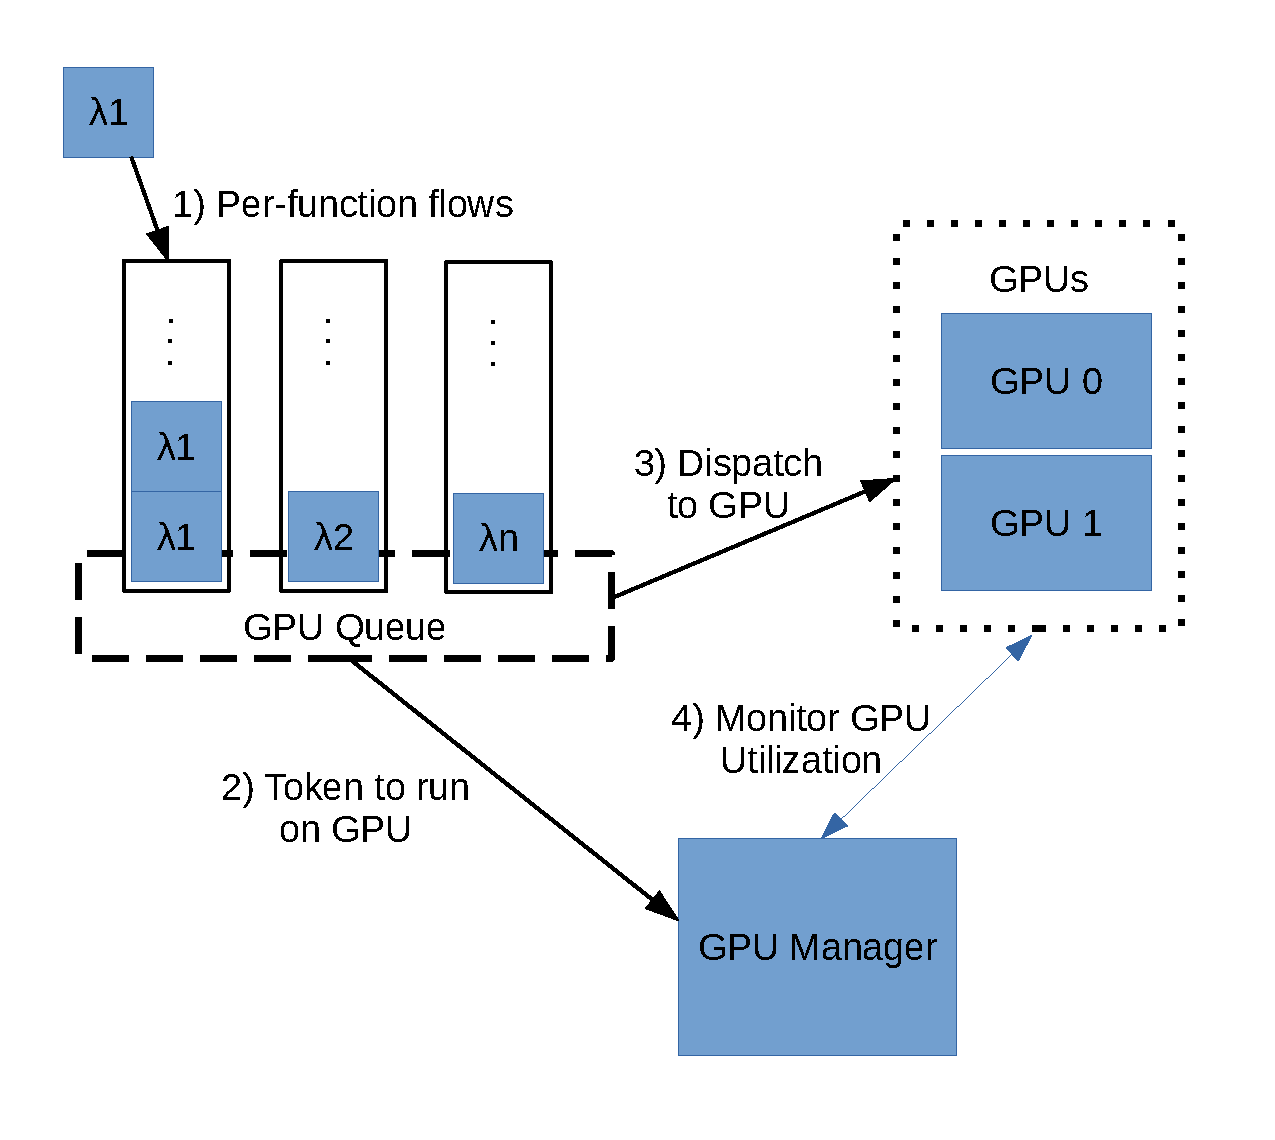
\includegraphics[width=0.45\textwidth]{../figs/queue-sys.pdf}
  \caption{\todo{Finalize Queuing/Driver/GPU-mgmt diagram}}
  \label{fig:sys-diag}
\end{figure}
